\section{Final Solution}
Our final solution is a stage-3 ensemble model trained with the multi-stage ensemble method described in Section 4.2 as follows:
\begin{itemize}
  \setlength\itemsep{0em}
  \item \textbf{Single Model Training}: First, we trained 64 single models with the 8 different algorithms and different subsets of 7 feature sets and DAE features.  Out of 64 models, there were 26 GBM, 14 NN, 12 FM, 6 LR, 2 KRR, 2 ET, 1 RF, and 1 KNN models.  Some of single models used RF feature selection, where we trained an RF model and selected features with high variable importances.
  \item \textbf{Stage-1 Ensemble}: Second, we trained 15 stage-1 ensemble models with different subsets of CV predictions of 64 single models.  Out of 15 models, there were 7 GBM, 4 NN, 2 LR, 1 FM, and 1 ET models.  Some of stage-1 ensemble models used rank orders between single models as additional inputs.  
  \item \textbf{Stage-2 Ensemble}: Third, we trained 2 stage-1 ensemble models with different subsets of CV predictions of 15 stage-1 ensemble models.  We used a LR with stepwise greedy forward selection and a GBM.
  \item \textbf{Stage-3 Ensemble}: Lastly, we trained a stage-3 ensemble model with CV predictions of all models.  We used LR with stepwise greedy forward selection, and it selected 5 models out of total 81 models: 1 stage-2 ensemble models, 3 stage-1 ensemble models and 1 single model.  Table 2 shows the list of models selected by the final stage-3 ensemble model.
\end{itemize}

Figure 6 shows the end-to-end pipeline for the final solution.  Details of the single and ensemble models trained are available in Table A3 and A4 in Appendix.

Our final solution achieved AUC scores of 0.90918 and 0.90744 on the public and private leaderboards respectively, and put us to the 1st place out of 821 teams.

At KDD Cup 2015, we made some observations as follows:
\begin{itemize}
\setlength\itemsep{0em}
\item As shown in Figure 5, our CV scores were very consistent with public leaderboard scores.  Therefore we used CV scores to determine (1) whether to add more ensemble stage or not and (2) whether to include a model for ensemble or not.
\item GBM outperformed other algorithms.  Our top 8 single models as well as top 2 stage-1 ensemble models are GBM models.  NN and FM were next best algorithms.  LR with stepwise greedy forward selection worked well in ensemble stages.
\item Biggest performance improvement was from the stage-1 ensemble, and as we added more ensemble stages, we observed diminishing improvements.  The stage-1, -2, and -3 ensembles improved the best CV score by 0.00967, 0.00028, and 0.000226 respectively.  However, it was the improvement from the stage-2 and -3 ensemble that allowed us to finish the 1st.
\end{itemize}

\begin{figure}[t]
  \centering
    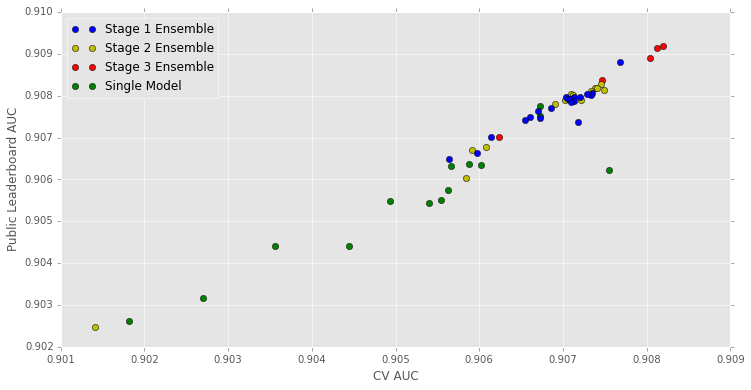
\includegraphics[width=0.5 \textwidth]{cv_lb}
      \caption{CV vs. public leaderboard AUC scores.}
\end{figure}

\begin{figure}[!t]
  \centering
    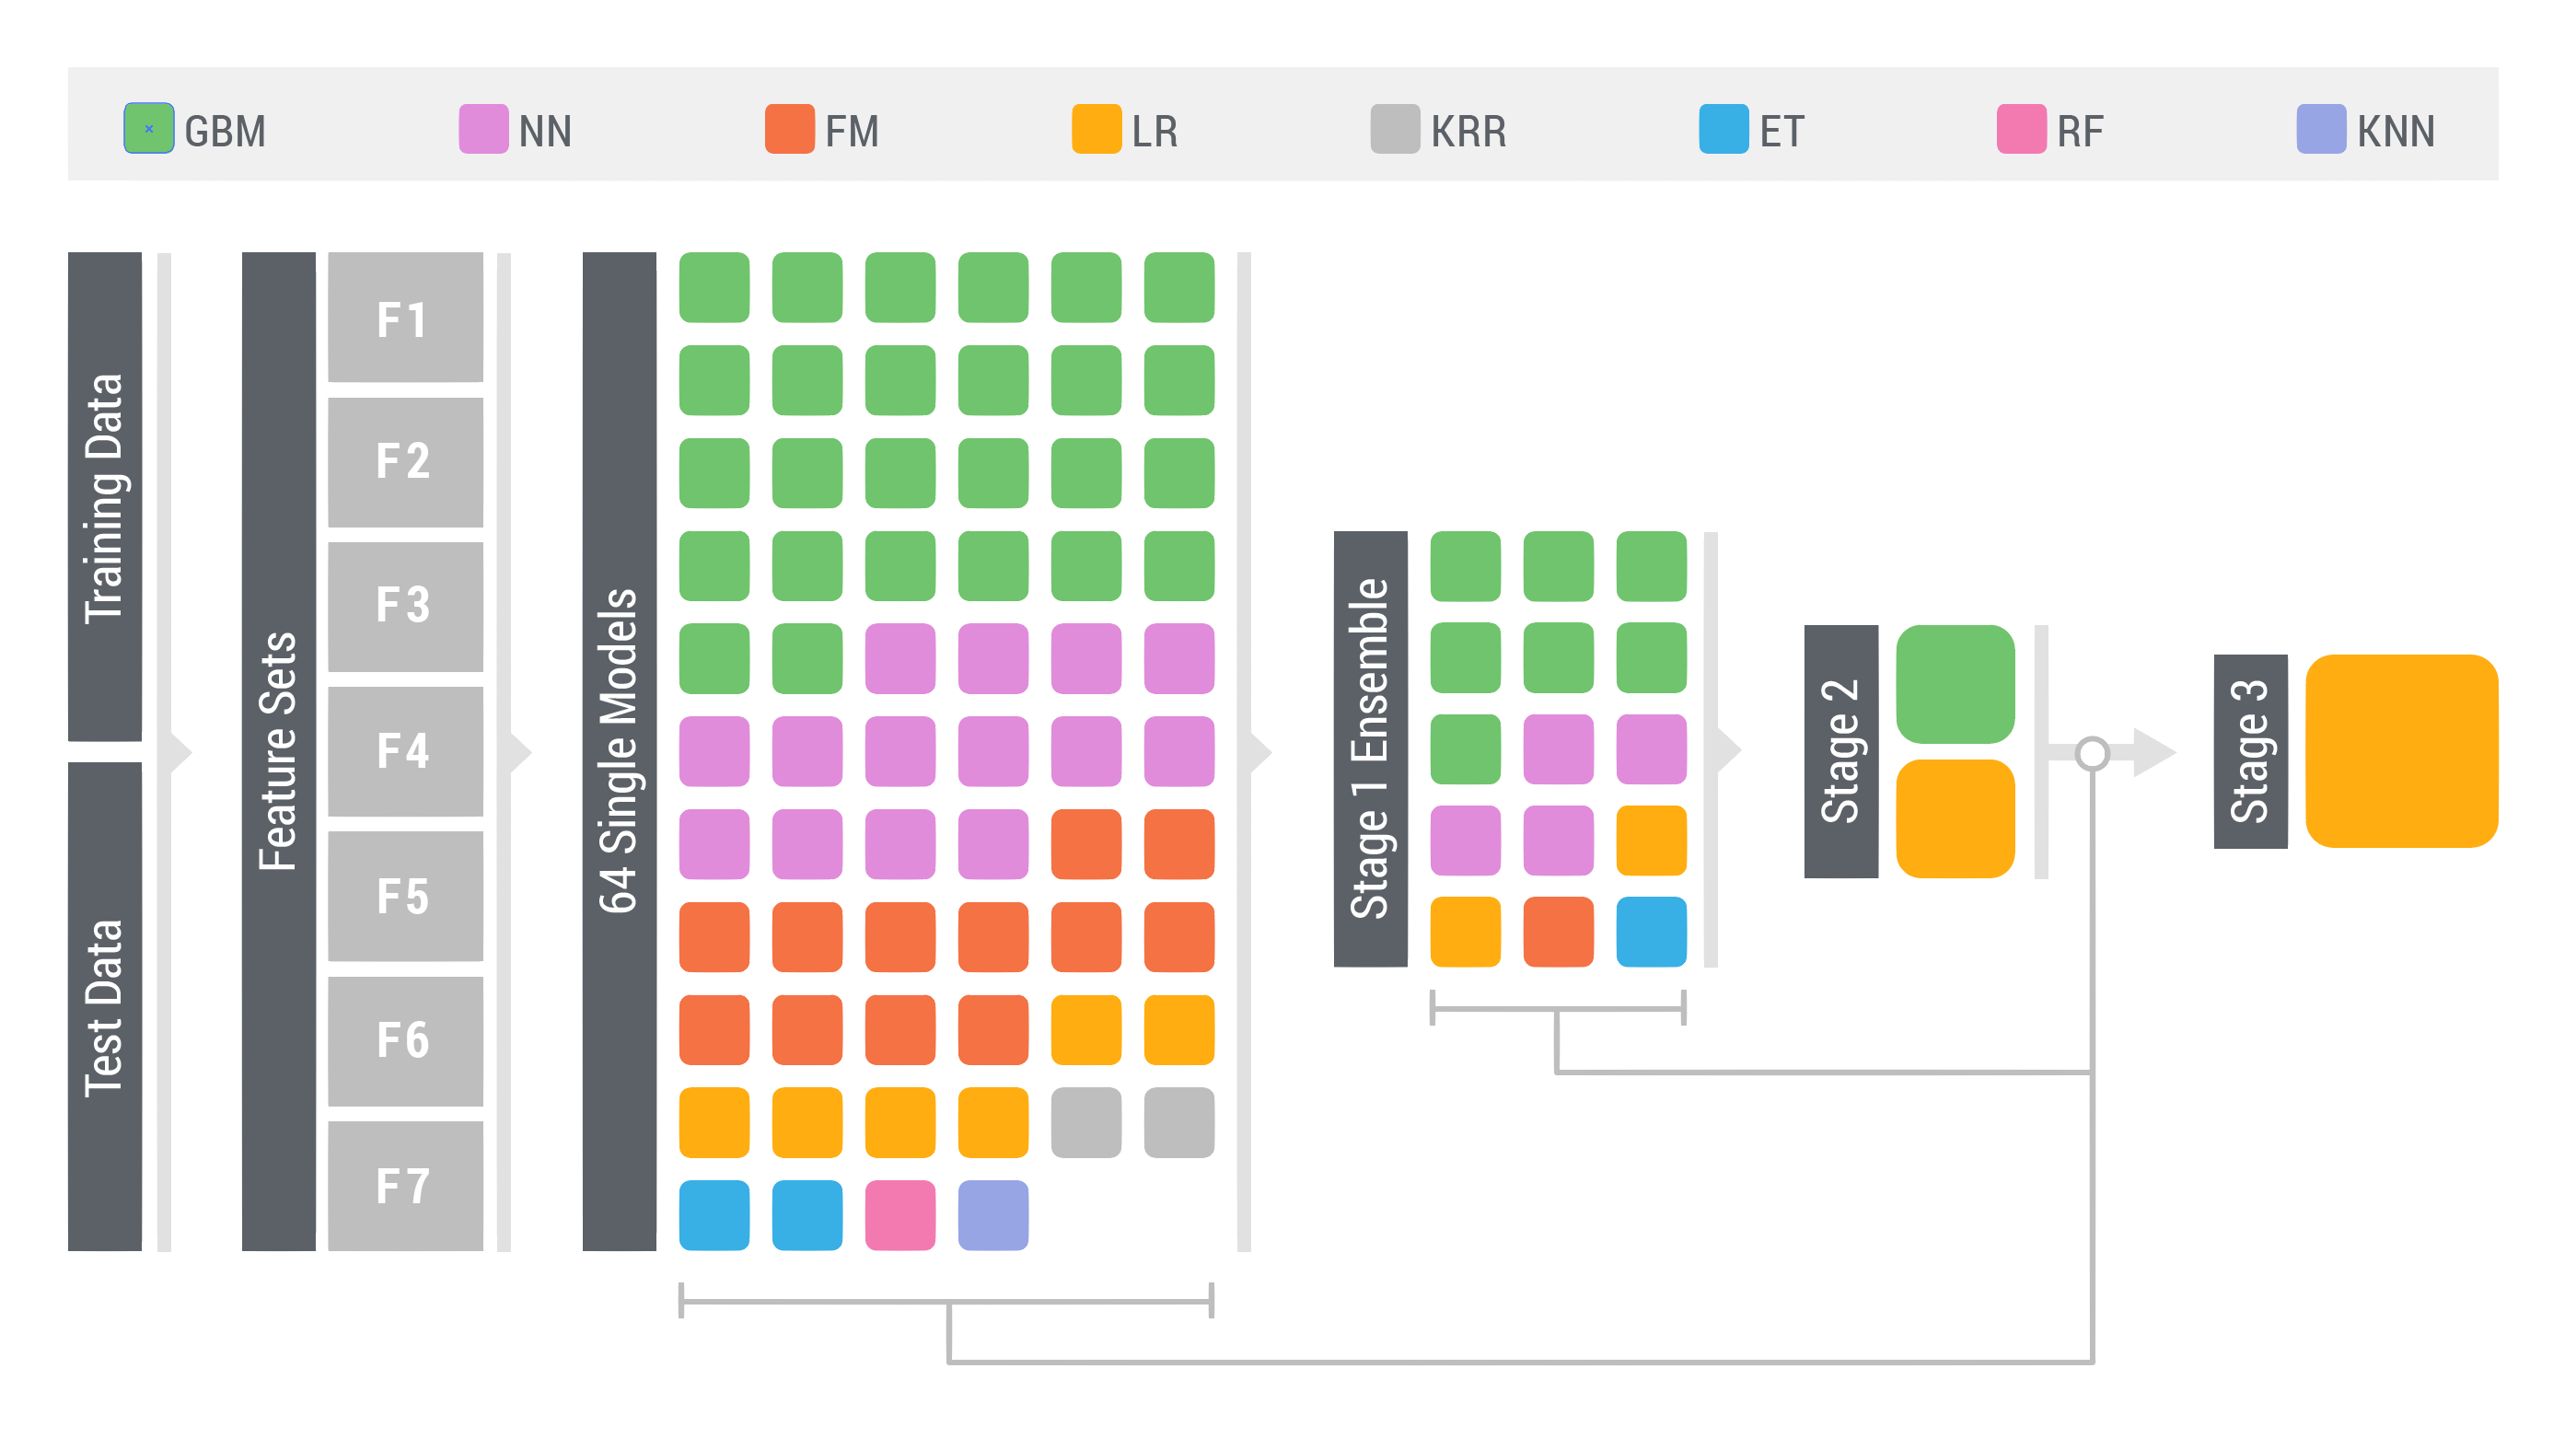
\includegraphics[width=0.5 \textwidth]{ensemble}
      \caption{End-to-end pipeline for the final solution}
\end{figure}

\begin{table}
\begin{center}
	\caption{Models selected in the stage-3 ensemble.}
\begin{tabular}{lllll}
ID 	& Stage 	& Algorithm 	& 5-CV 		& Weight\\ \hline
S1 	& Single	& GBM		& 0.906721 	& 1.1703 \\
E4 	& 1 		& GBM		& 0.907878 	& 1.9626\\
E8 	& 1 		& NN		& 0.907567	& 0.7871\\
E18	& 1		& ET			& 0.906207 	& 0.4580\\
E2	& 2 		& LR			& 0.907968 	& 1.6146\\
\end{tabular}

\label{tb:finalEnsemble}
\end{center}
\end{table}
